\chapter{Friction estimation method}

This chapter will describe the chosen method that has been used to estimate the tire/road friction. Different approaches are weighted where a great deal of effort has been put on dealing with the fact that the method should work well in a practical manner, rather than during simulations.

\section{Approach}
The main idea for how to estimate friction is the following. Two models describing the vehicle forces and the tire forces are used. The next step is to make sure that all parameters for the vehicle model is known and that all parameters for the tire model except the tire/road friction coefficient is known. Finally, by fitting the tire model to the vehicle model with recursive least square fitting, using the tire/road friction coefficient as fitting parameter, the tire/road friction coefficient can be estimated. This is true because the forces generated by the tires should be equal to the total force acting on the vehicle.

The first step of the method include calculations of the forces acting on the vehicle by using a vehicle model. This is for example done by using measured and calculated parameters such as wheel speed, yaw rate and acceleration but it can be done in other ways as well. Two different models that describes the vehicle forces will be presented in this work. 

The second step is to calculate the forces generated by the tires through a tire model. Such a model often depend on the tire stiffness, the tires slip ratio, the normal force acting on the tire and the road friction coefficient. Several tire models exists today and in this work three of them will examined more closely. It's in combination with the tire force calculations that the recursive least squares fitting is executed as well. This will also be explained in more detail. 

\subsection{Practical restrictions and problems}
The idea presented above might sound like a very simple solution but there are several problems that have to be considered. The most important aspect that has to be taken into account is the fact that the friction estimation model has to work in a real car handled in actual driving situations. In a theoretical world, where a vehicle and a tire model is fed unbiased data, the friction coefficient can be obtained with good certainty and quite fast. Unfortunately, in the practical world, the data fed to the models are far from optimal. Things like measurement noise and approximative calculations corrupts the results. Several more complex driving situations are also hard to model correctly. This can for example be excessive wheel spin, aggressive cornering or speeds close to zero.

The true dynamics of both a vehicle and a tire is very complex and therefore also difficult to describe accurately with a model. At the same time, a model that is to be used has to be simple enough so that calculations are possible on an micro control unit with limited computational power. Even though many simplified models are shown to be accurate enough to reflect reality in most driving situations, there are times when a simplified model inaccurately describes the detailed dynamics of a vehicle or a tire. 

There are also numerous models that use parameters which are hard to measure or approximate well in reality. Some of these parameters include the lateral velocity and slip angle. It is therefore desired to have a model that doesn't rely on these parameters. There are also car specific parameters, some which change between driving sequences, that can have a large impact on the modeled results. A few of these parameters include the mass of the vehicle, wheel radius, wind drag coefficient, lengths from center of gravity to the rear and front axle and the center of gravity height. When using simulations, the exact value of these parameters can be known, but in a real environment they either have to be static, approximated or neglected in computations.

\subsection{FXD}
The problem stated in this work is to estimate the tire/road friction for a car using an FXD. This results in a number of conditions that have to be thought of and applied throughout the research. First of all, cars with an FXD installed are solely front wheel driven, meaning that there are no positive longitudinal forces acting on the rear wheels. The velocity of the rear wheels can therefore in most cases be used as a good approximation of the vehicles reference speed. Through the same reasoning, the longitudinal acceleration of the car can be derived from the derivative of the rear wheel velocities. There is also no steering done by the rear wheels.

Another aspect that has to be considered is that the FXD is an active limited slip differential, which means that the torque applied to the two driving shafts can differ in certain situations, unlike a car equipped with a standard open differential.

\subsection{Related work}
There have been quite extensive amount of research within this field of study and many different model proposals related to friction estimation during the last decades. The outcome of these researches usually show promising results, where the proposed solution works well during simulations and/or testing. Related work has provided a lot of information and help to this work, especially when it comes to getting a general understanding of the problem and its difficulties. But due to the fact that many results are based on theoretical simulations, a lot of information could be of little use or in some cases even be misleading.

\subsection{Conclusion}
All in all it is a great challenge to estimate the tire/road friction coefficient. \todo{Make sure this is true.} The approach, all of the problems mentioned and how they were taken care of will be explained in greater detail later on in the report.

\section{Signal processing}

Apart from the fact that a vehicle is hard to model properly, the parameter signals from the vehicles CAN bus are noisy and can also be delayed.

\subsection{Filters}

Apart from the fact that a vehicle is hard to model properly, the parameter signals from the vehicles CAN bus are noisy and can also be delayed. It order to get a more exact instantaneous value, without noise, these signals need to low pass filtered. 


\subsubsection{Timing of signals}

Due to filtering (multiple filtering(acc)), signals delayed, have to be timed.

Different signals have different noise, and therefore should be filtered differently, this leads to signals being delayed against each other. 

\subsection{Static parameter impact}

Massa, radie på hjulen, CGO height, osv..

\section{Vehicle forces}
There are several forces acting on a vehicle. The largest forces are generated between the tires and the ground because the tires are the only parts of a car that have any physical contact with the surrounding world. While accelerating and braking longitudinal forces will arise and while cornering lateral forces will arise. The tires are responsible for all the forces that actually control the vehicle which makes them very important for good handling but also makes them hard to model. Beside these major forces there are also forces such as wind drag and rolling resistance acting on the vehicle.

The trick is to calculate all the forces into one total force that can be compared to the total force generated by the tires.
\subsection{Vehicle force calculated from longitudinal acceleration}
The simplest way of representing the force acting on the vehicle while accelerating is to use the acceleration and the mass of the car and apply Newtons second law of motion:
\begin{equation}
	F = m \cdot a
\end{equation}
\subsubsection{Estimating the longitudinal acceleration}
\label{longaccest}
For this method to be accurate an accurate estimation of the longitudinal acceleration is needed. Some cars have accelerometers installed for longitudinal measurements which makes it straight forward to calculate the force. If one of those aren't available the acceleration has to be calculated instead. This can be done by derivation of the vehicles speed. The speed of the vehicle can be obtained by measuring the speeds of the undriven wheels. For a FWD car this would be the rear wheels. To make the calculation more accurate the average speed of the two rear wheels is calculated before the derivation is done.
\begin{equation}
a_{x} = \frac{d}{dt}(\frac{w_{rl}+w_{rr}}{2})
\end{equation}

\subsubsection{Estimating the losses}
Two different losses are compensated for. Losses from drag and losses from rolling resistance.

The drag force is calculated as:

\begin{equation}
F_{D}=\frac{1}{2}\rho v^2 C_{d}A
\end{equation}
where:
\begin{itemize}
	\item $ \rho $ is the density of air.
	\item $ v $ is the speed.
	\item $ C_{d} $ is the drag coefficient.
	\item $ A $ is the cross sectional area.
\end{itemize}
The rolling resistance is calculated as in Equation \ref{eq:rollingres}.

\subsubsection{Estimating the total vehicle force}
The total amount of force acting on the vehicle thus becomes: \todo{this formula might be altered}
\begin{equation}
\label{eq:newton}
F_{vehicle} = m \cdot a + F_{drag} + F_{rolling resistance}
\end{equation}

\subsubsection{Complications}
The main issue with this method is that it's based on longitudinal acceleration and longitudinal losses only, hence it can only be used to estimate the vehicle forces when accelerating in a straight line. Although this is a big restriction it might be enough since acceleration in a straight line happens pretty often while driving.

A major hardship is to obtain a proper value for the longitudinal acceleration. If the vehicle doesn't have an accelerometer the acceleration calculated from the wheel speeds needs to be used. This immediately causes problems when the vehicle is accelerating on a gradient road. During an uphill acceleration, the actual force to accelerate the vehicle will be higher than the force calculated from Newtons second law. Driving downhill, the force will be lower. This is because the earths gravity isn't considered in the formula. When climbing a hill the vehicle force needs to include the force of the earths gravitational pull as well. The same goes for then driving downhill, but now the force will instead help accelerating the vehicle. The force of the gravitational pull can be calculated if the angle of the vehicle relative the earths horizontal plane is known but this angle is hard to measure or estimate. \todo{is it really?}

Measuring it with an accelerometer ......\todo{does it work good or bad in hills?}

The second parameter of Newtons second law is the mass which also is hard to estimate. The mass of the vehicle can vary several hundreds of kilos depending on passengers and load in the trunk. A Golf GTi has a curb weight of about 1350 kg. Hence, the varying weight of several hundreds of kilos will have a great impact on the force calculations. To counter this problem some kind of load detection needs to be available to set a new mass every time the car is driven. This isn't something that is very common on cars today and thus a static mass of the vehicle needs to be set resulting in errors in the force calculations way too often.

Suppose that the force calculation from Newtons second law is correct. Still there are losses to be accounted for. They need to be calculated properly to be able to compare the vehicle force to the tire force. Looking at the formula above \ref{eq:newton}, two different losses are compensated for. The rolling resistance is straight forward if the rolling resistance coefficient is known. The drag is a bit more complicated but should prove to be fairly accurate as well if the parameters is known. All in all, the results of these calculations won't be perfect and there are several more losses that can't be calculated in any good way. \todo{are there really?}


\subsection{Vehicle force calculated from engine torque}
Another way of calculating the longitudinal force of a vehicle is to derive the actual torque that is applied to the shafts connected to the driven wheels. The advantage of using the engine torque, instead of the acceleration of the vehicle, is its independence of the roads gradient and losses such as wind drag and steering losses. The torque that is applied to the shafts will be directly proportional to the actual force generated by the wheels, regardless of how the gravitational pull and other losses are acting on the vehicle. 

The formula for calculating the total torque on the drive shafts is simple:
\begin{equation}
\label{eq:tshaft}
T_{driveshafts} = T_{engineshaft}\cdot GearRatio
\end{equation}
where the gear ratio is the speed ratio between the engine shaft and the differential housing:
\begin{equation}
\label{eq:GR}
Gear Ratio = \frac{RPM_{engine}}{RPM_{diffhouse}}
\end{equation}
and finally the speed of the differential housing is the average speed of the left and right drive shafts:
\begin{equation}
\label{eq:diffhouse}
RPM_{diffhouse} = \frac{RPM_{leftdriveshaft}+RPM_{rightdriveshaft}}{2}
\end{equation}
The engine torque, engine speed and the drive shaft speeds (wheel speeds) are all parameters commonly found on the CAN bus of a newer car. Important to notice is that these calculations do not consider any losses from the engine to the drive shaft. By combining equations $ \ref{eq:tshaft} $ and $ \ref{eq:GR} $, it is seen that the power generated by the engine and the power outputted to the drive shaft are equal.
\begin{equation}
P = T_{driveshaft}\cdot RPM_{driveshaft} = T_{engineshaft}\cdot RPM_{engineshaft}
\end{equation}

The torque will be split evenly between the two drive shafts, assuming an open differential, i.e. when the FXD is inactive. If the FXD is active the available torque on the drive shafts has to the redistributed according to the amount of torque being transfered through the FXD. This is important to consider if force calculations for a single wheel are to be done.   

When the torque on each drive shaft is calculated the force acting on each tire is calculated by dividing that torque by the wheel radius:
\begin{equation}
\label{eq:tireforce}
F_{tire} = \frac{T_{shaft}}{R_{e}}
\end{equation}
These forces can then be compared to the forces generated by the tire models for each tire.

\subsubsection{Gear ratio}
Calculating the gear ratio with Equations \ref{eq:GR} \& \ref{eq:diffhouse} gives varying results. Both the engine speed and wheel speed signals are noisy. In the gear change moment it will take some time for them to stabilize again resulting in long times of faulty force calculations. 

On newer cars it's not very uncommon to find what gear is active at the moment as a signal on the CAN bus. By knowing this the gear ratio can be set without any calculations since the gear ratio for each gear is known. For the Golf GTi the gear ratios can be seen in Table \ref{tab:gr}. A graph of the calculated and predefined gear ratio can be seen in Figure \ref{gear_ratio}. It can be seen that the calculated signal is much slower than the predefined one. It's also oscillating quite much which is bad because the gear ratio really is a static value purely depending on what gear is active. 


\begin{table}[position specifier]
	\centering
	\begin{tabular}{| l | l |}
		\hline
		Gear & Gear ratio \\ \hline
		1 & 13.9284 \\ \hline
		2 & 8.5383 \\ \hline
		3 & 5.4378 \\ \hline
		4 & 3.7206 \\ \hline
		5 & 2.7666 \\ \hline
		6 & 2.1942 \\ \hline
	\end{tabular}
	\caption{Gear ratios for the Volkswagen Golf GTi Mk7}
	\label{tab:gr}
\end{table}

\begin{figure}[h]
	\centering
	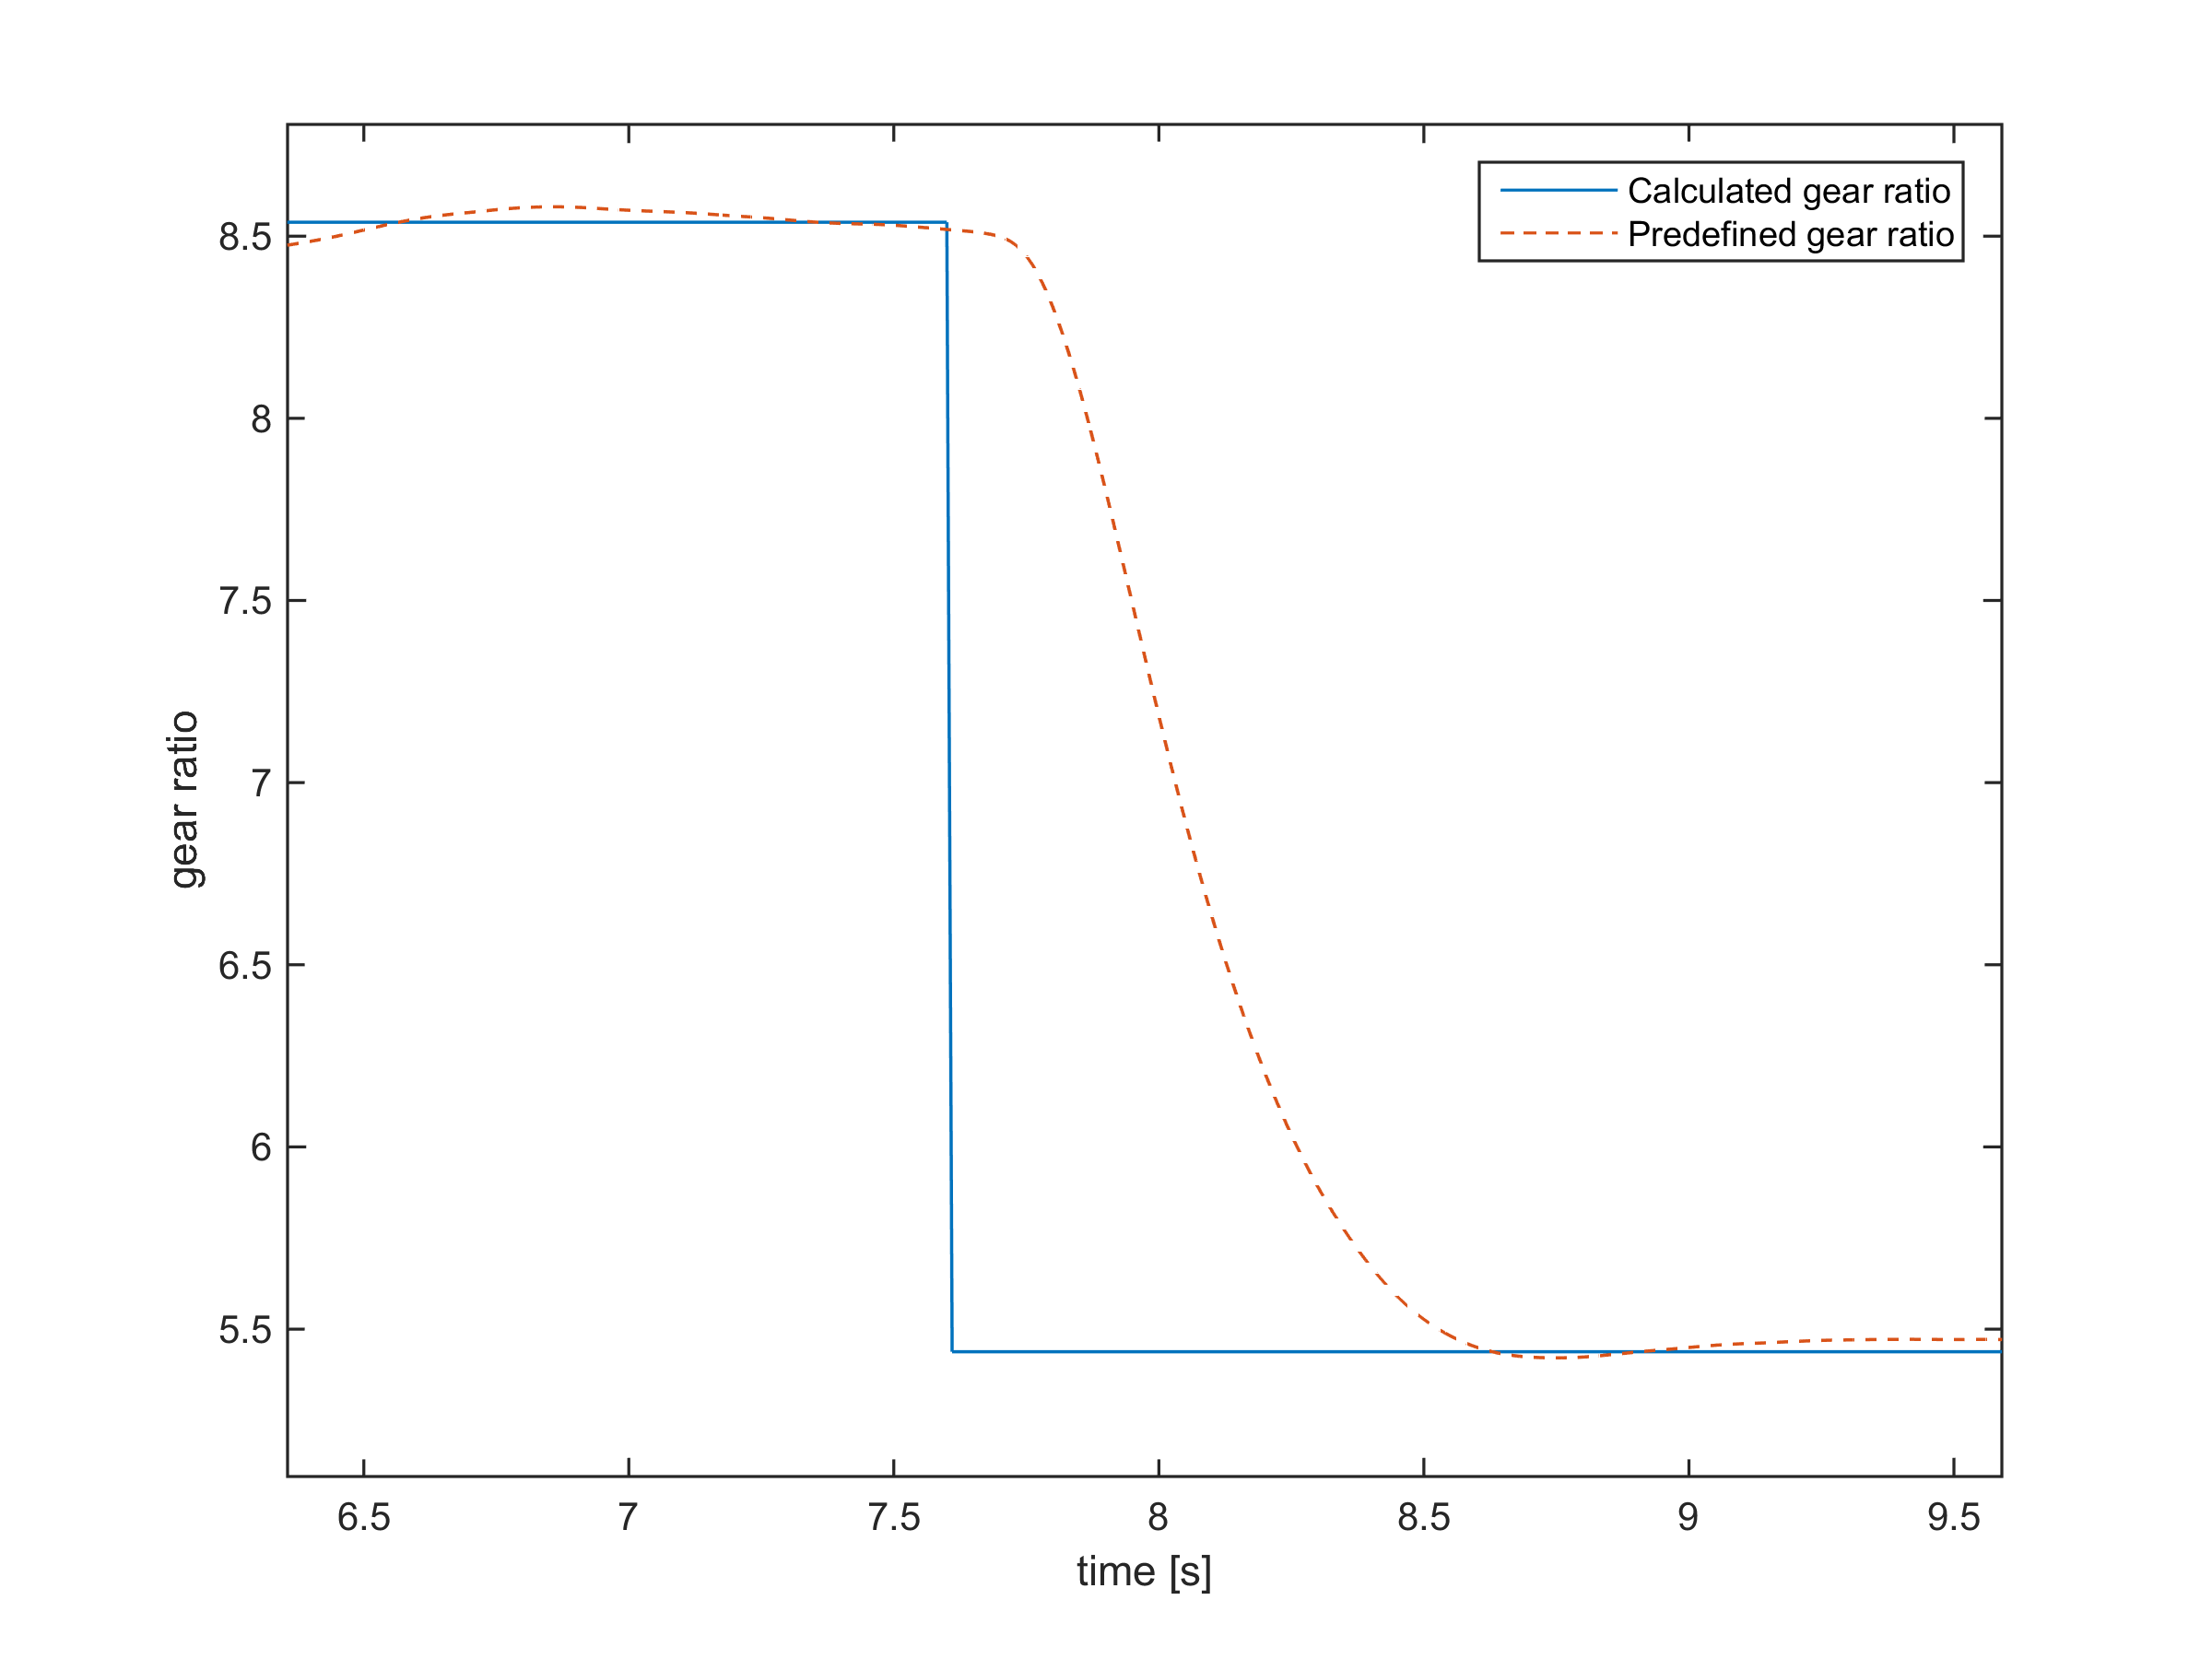
\includegraphics[width=0.8\textwidth]{Pictures/gear_ratio}
	\caption{Calculated and predefined gear ratio in a gear change from 2nd to 3rd gear.}
	\label{gear_ratio}
\end{figure}

\subsubsection{Transfer losses}
There are several factors that affect how much of the engine torque that actually becomes available on the drive shafts. There are several losses in a drive line. Friction and rotating masses within the drive line are the main contributors. Some torque are also lost accelerating the mass of the wheel itself.
\begin{equation}
T_{driveshaft} = T_{driveshaftwithoutlosses}\cdot\eta_{friction}\cdot\eta_{rotating mass} - T_{wheelacceleration}
\end{equation}
$ \eta_{friction} $ is just a scalar factor. The frictional losses are very dependent on the design of the drive line. This means that the losses will differ between vehicles and that this factor needs to be calculated for each specific car model. Since this factor is easy to change it will also include other losses in the drive line such as acceleration of the drive shafts. \todo{can we say this?}

$ \eta_{rotating mass} $ is modeled as:
\begin{equation}
\eta_{rotating mass} = \frac{1}{1 + factor(0.0025?)\cdot gearratio^2}
\end{equation}\\
\todo{choose factor}
The efficiency gets worse as the gear ratio gets higher since there will be more rotating mass in low gears. \todo{is this true?} Just as the frictional losses this loss is also dependent on the design of the drive line. Thus the factor multiplied with the gear ratio needs to be decided for each specific car model.

To calculate $ T_{wheelacceleration} $ requires some more steps. Each wheel connected to a driven shaft has its own moment of inertia which will be accelerated if enough torque is applied. The amount of torque needed to accelerate the wheel depends on its moment of inertia and the angular acceleration:
\begin{equation}
	T = a \cdot I
\end{equation}
The moment of inertia is the wheels radii squared and integrated over the mass. 
\begin{equation}
	I = \int r^2 \cdot dm
\end{equation}
Assuming that a wheel has the shape of a solid cylinder with equal amount of density throughout, the moment of inertia for a wheel can instead be described as:
\begin{equation}
	I = \dfrac{r^2 \cdot m}{2} 
\end{equation}
In the same manner, this applies for the actual drive shafts as well but as was said earlier this loss is included in the scalar factor describing the frictional losses. \todo{again, can we say this?}

The angular acceleration is calculated in the same manner as in Section \ref{longaccest} but now for the front left and right wheel separately.
\subsubsection{Complications}
This method includes some negative aspects that have to be thought of. It is unfortunately very uncommon for a commercially available vehicle today to have a torque sensor mounted, which means that the torque has to be obtained with other parameters. The torque applied to driving shaft is simply the torque generated from the engine multiplied by the current gear ratio.

A restriction that has to be thought of is that the amount of force that can be generated between the tire and the road is limited by the tire/road friction and the normal, $ \mu \cdot F_{z} $. Any additional torque applied to the shaft will add to $ T_{wheelacc} $ and merely serve as unwanted acceleration of the wheel, i.e. spinning.

\section{Tire forces}
To calculate the tire force properly the slip angle is needed. 

The characteristics of a tire is very complex, which makes the actual forces generated to the vehicle  difficult to obtain. The main dynamic parameters of existing longitudinal tire force models include the slip ratio, normal force, and the tire/road friction coefficient, $ \mu $:
\begin{equation}
F_{tire, longitudinal} = f(\kappa, Fz, \mu, C_{x})
\end{equation}
The slip ratio is calculated from the wheels difference in angular and forward velocity as seen in equation $ \ref{eq:longslip} $, the normal force from the weigh of the vehicle and the changing weight distribution derived (IN PREVIOUS CHAPTER), and the tire stiffness as explained  in (IN PREVIOUS CHAPTER). Thereafter, the only dynamic parameter of the tire force equation becomes the friction coefficient. By choosing the correct $ \mu $, the force from the tire model will equal the force from the vehicle model. This calculation is done in a feedback manner, meaning that the tire force depends on the friction coefficient derived in the previous iteration.

\begin{figure}[h]
	\centering
	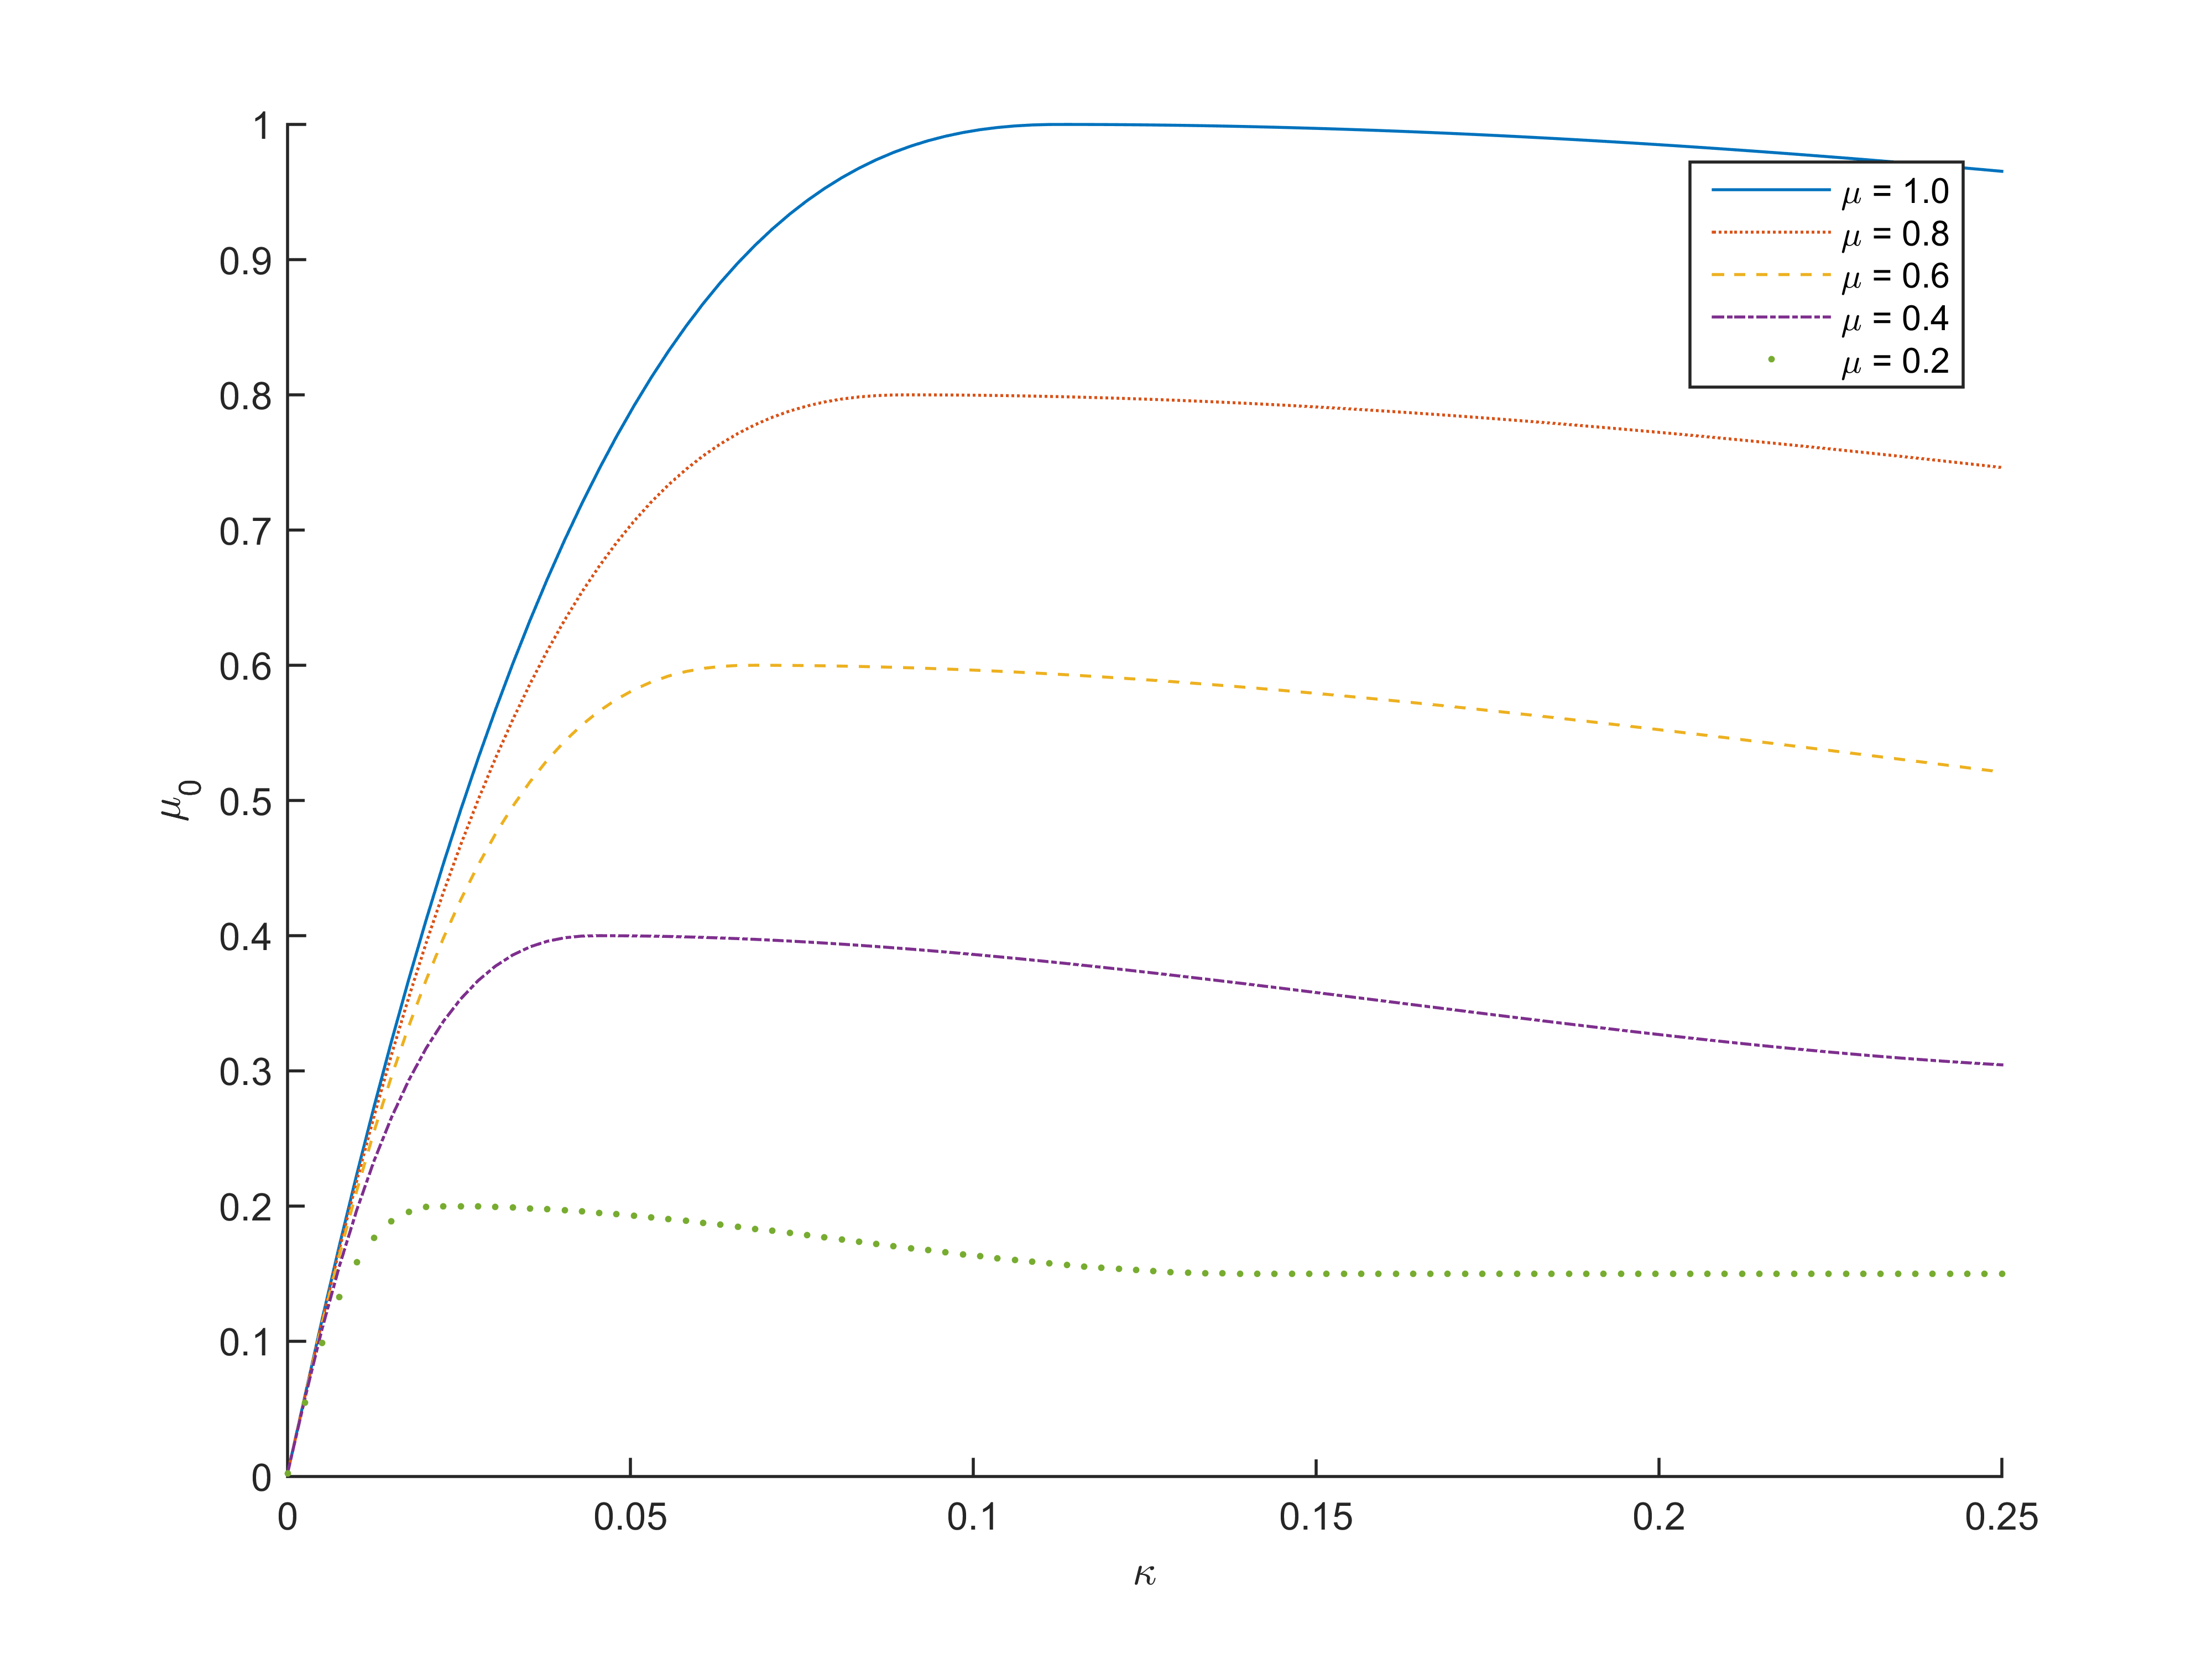
\includegraphics[width=0.8\textwidth]{Pictures/slipkraft_olika_mue}
	\caption {Normalized tire model force per slip ratio for different  mue values.}
	\label{different_mue}
\end{figure}


\subsection{Tire stiffness}

The tire stiffness is obtained by deriving the tire force generated per slip for values around zero, e.i. the gradient of the slip/force curve at zero slip. The slip force curve for two different tire stiffness's can be seen in \ref{different_cx}. The interpretation from this figure is that a tires stiffness is an essential parameter to have in order to model the tire force correctly. 

\begin{figure}[h]
	\centering
	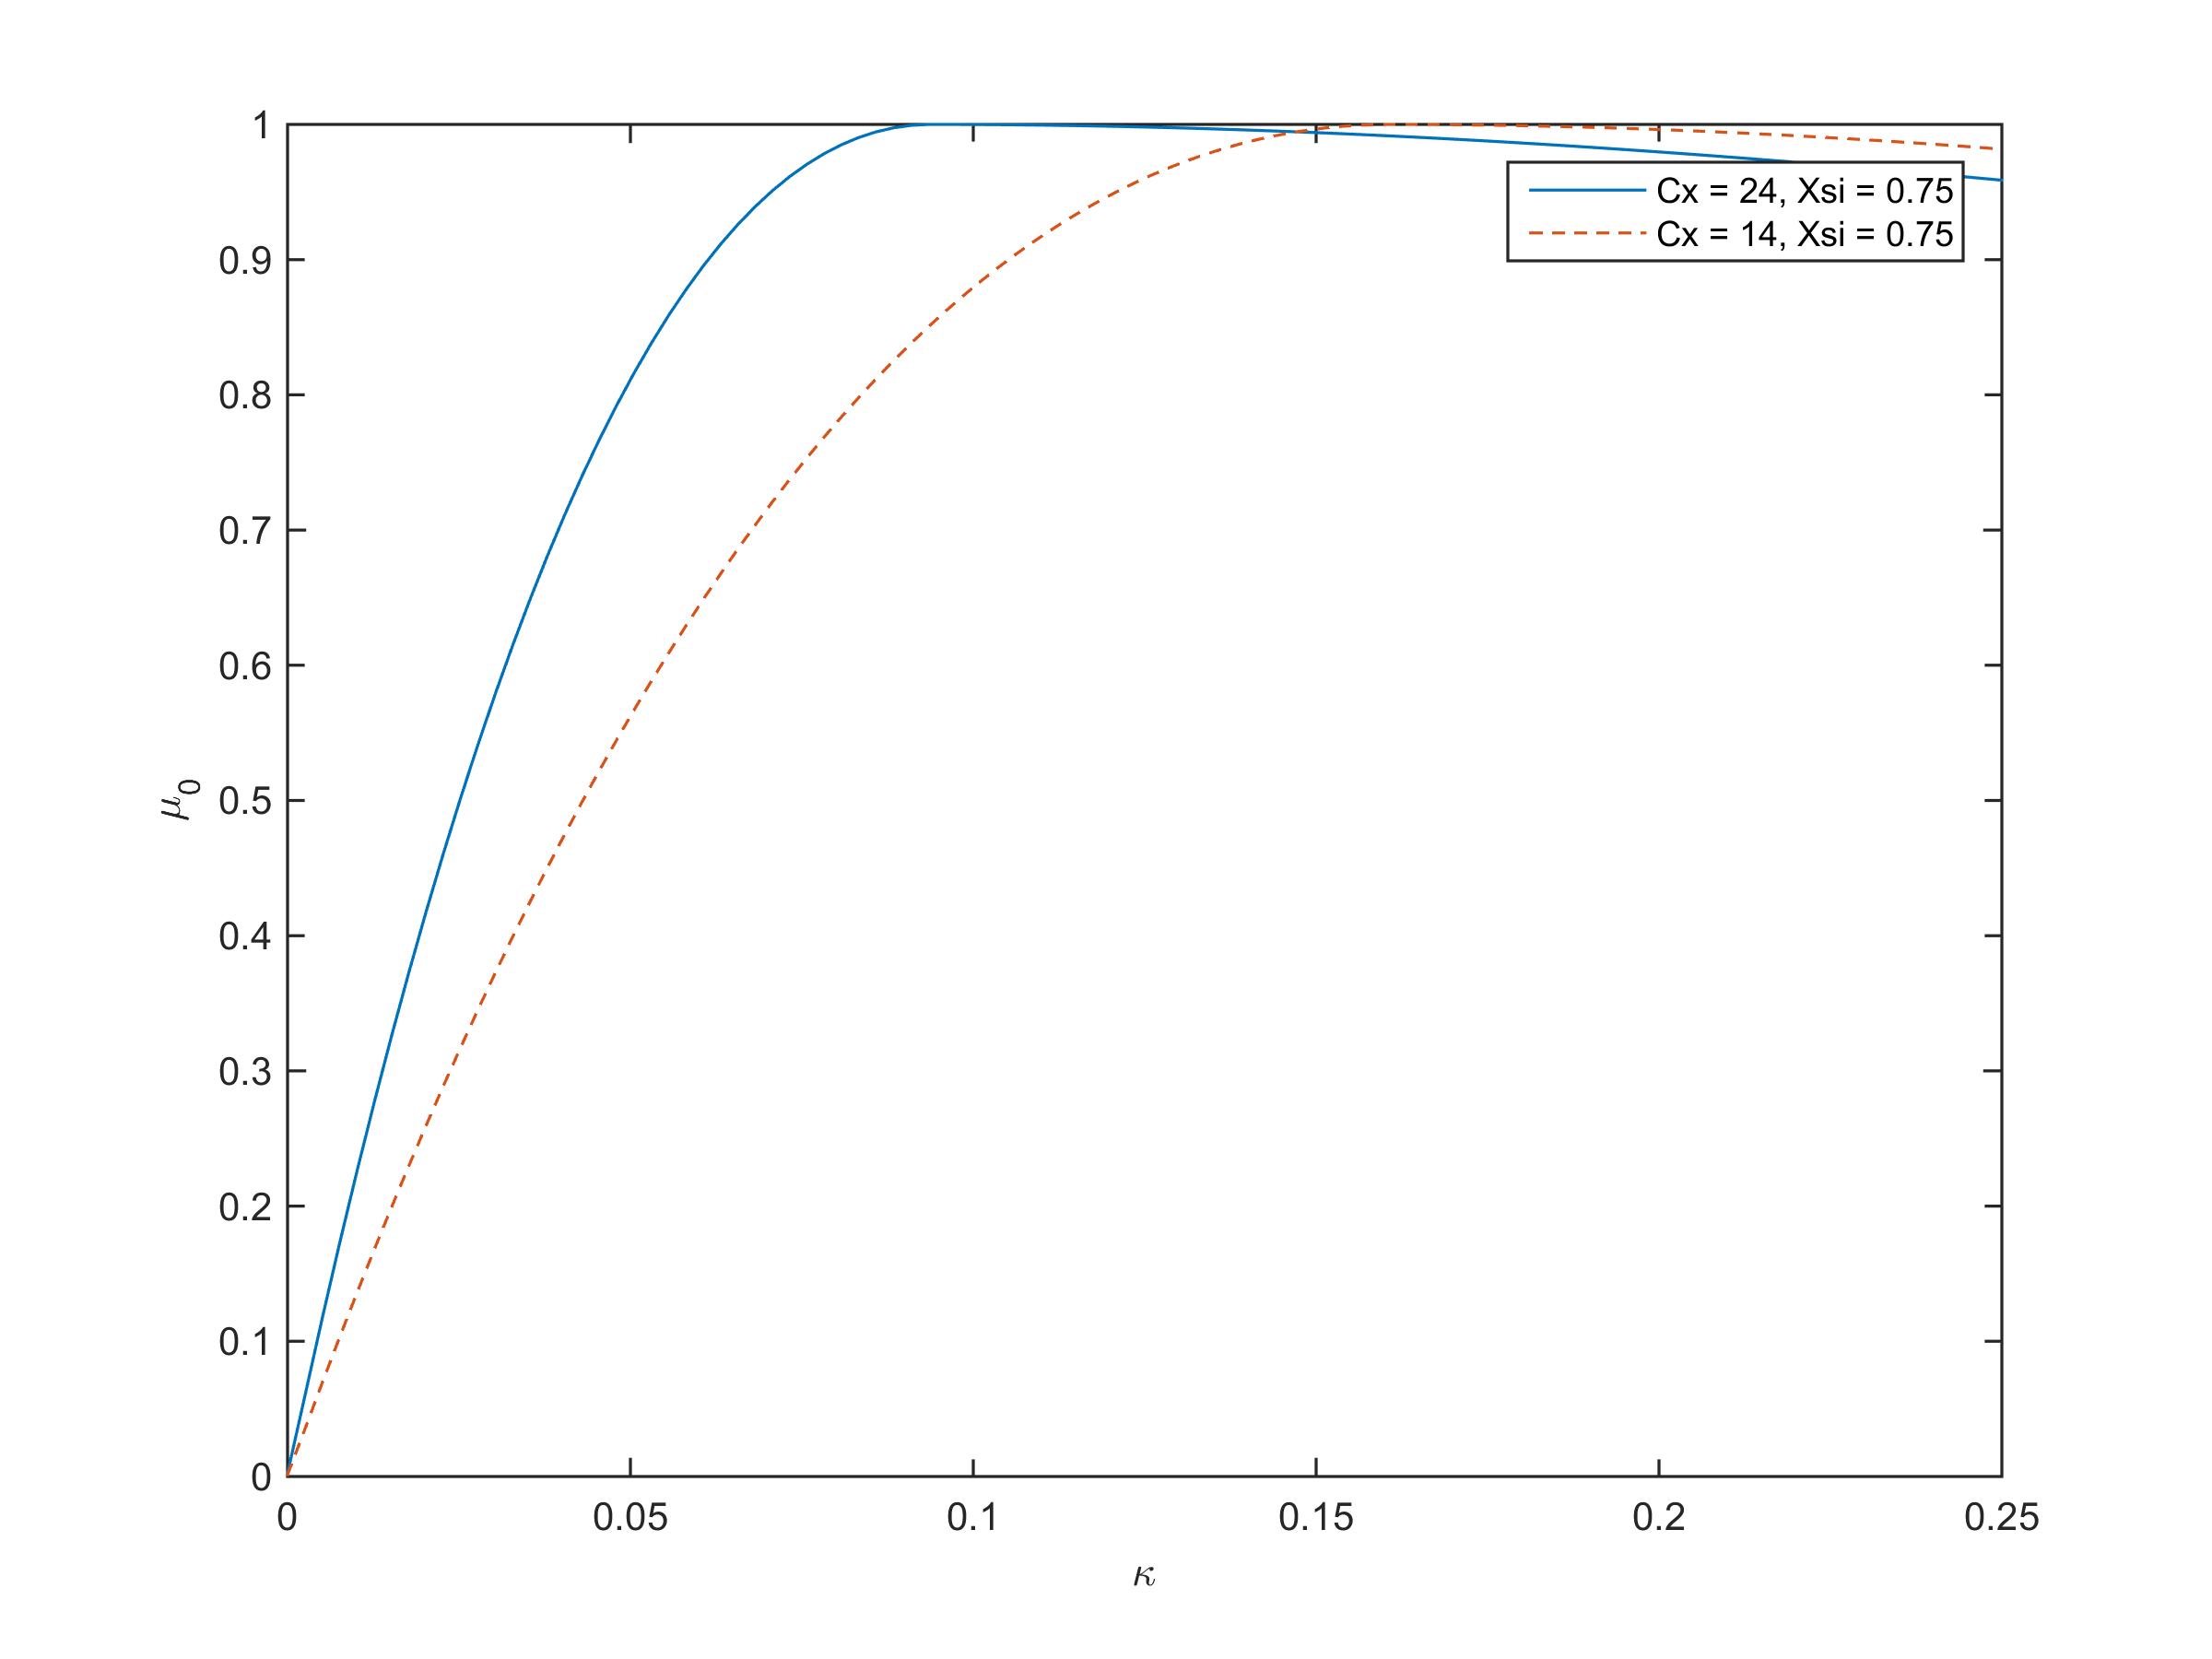
\includegraphics[width=0.8\textwidth]{Pictures/slipkraft_olika_cx}
	\caption {Normalized tire model force per slip ratio for different tire stiffness's. $ \mu = 1.0 $.}
	\label{different_cx}
\end{figure}

Unfortunately, a tire characteristics is further complex, and cannot be explained by the tire stiffness as a parameter alone. Two different tires can have the same tire stiffness, but differing characteristics at larger slip ratio values. An example of this can be seen in \ref{different_xsi}. Generally, tires with lower tire stiffness value have higher Xsi, hence resulting in even lower forces for higher slip values (IS THIS EVEN TRUE???). 

\begin{figure}[h]
	\centering
	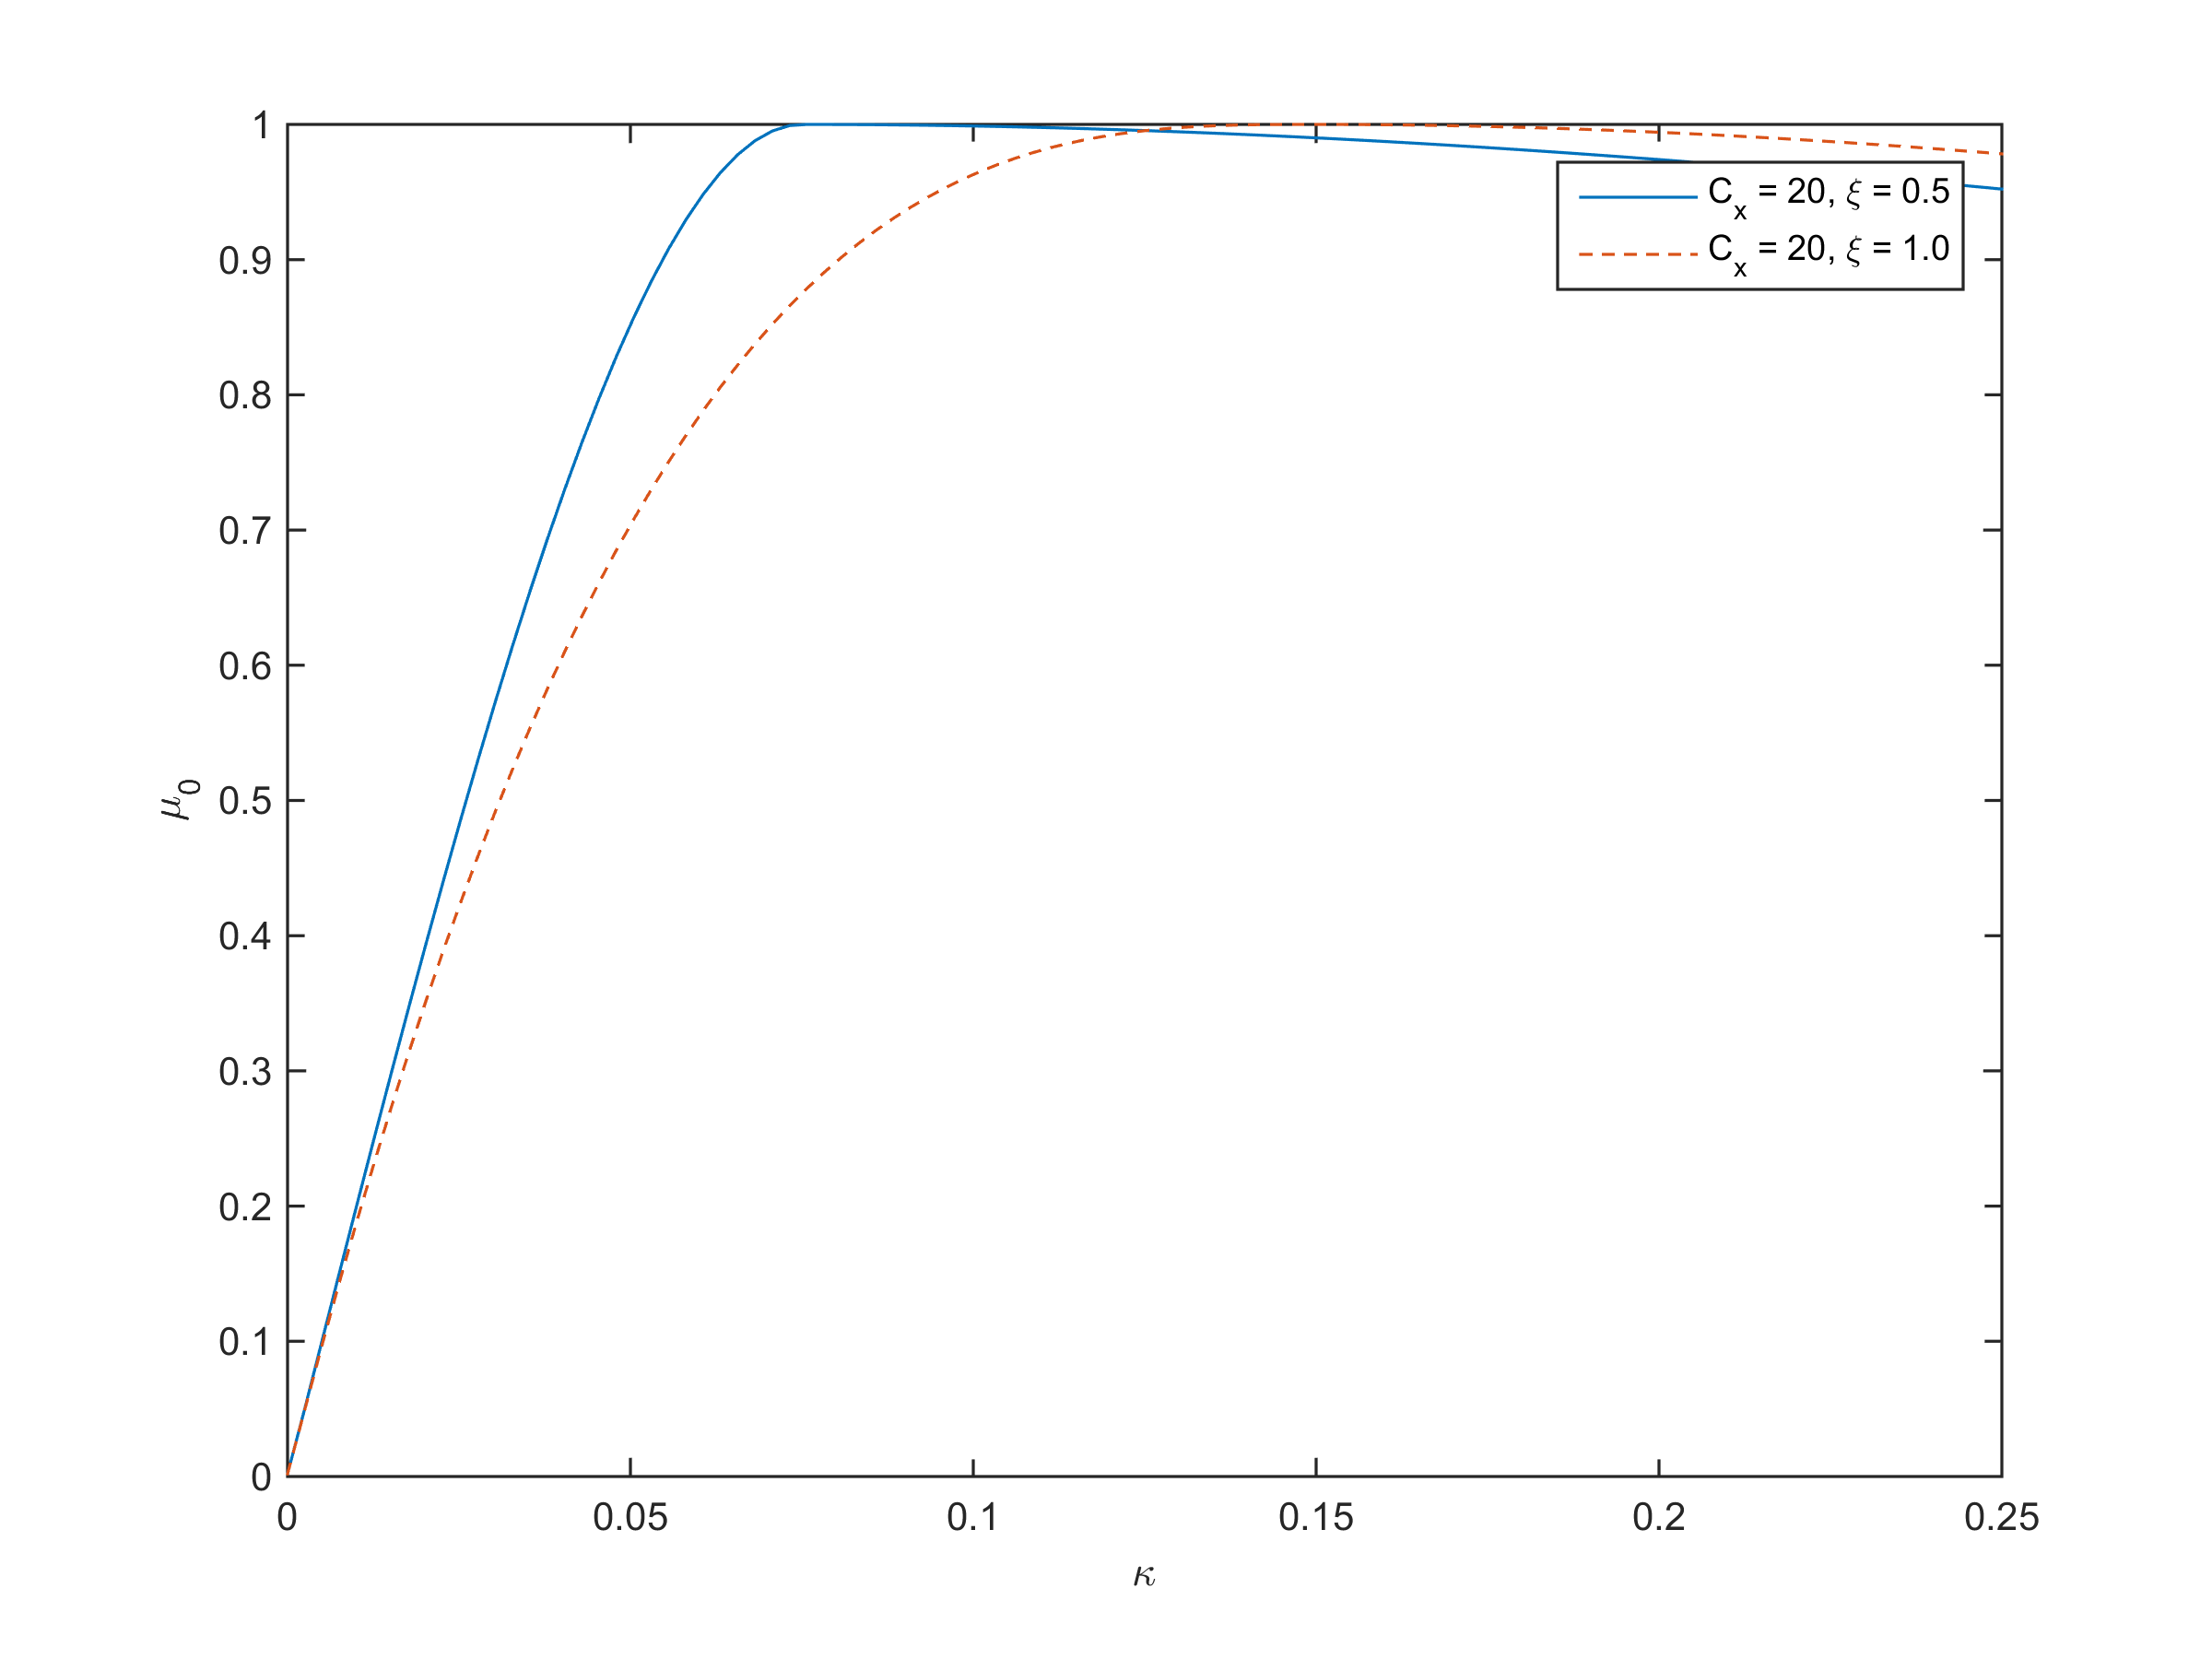
\includegraphics[width=0.8\textwidth]{Pictures/slipkraft_olika_xsi}
	\caption {Normalized tire model force per slip ratio for different tire characteristics for higher slip ratios.  $ \mu = 1.0 $.}
	\label{different_xsi}
\end{figure}

The tire stiffness for a certain tire should theoretically be the same for different road surfaces. Nevertheless, testing has shown that the actual inclination of the slip/force curve for small slips can differ for different road surfaces. The tire stiffness therefore has to be compensated accordingly depending on the roads friction coefficient.

\subsection{Slip ratio}

As seen in most slip/force figures, the maximum force will be generated at a specific slip and will thereafter decrease with an increasing slip ratio. If the tire model doesn't capture this force peak at the correct slip ratio value, it will become very difficult to match the tire model force with the calculated vehicle force. The slip ratio value during a real driving sequence is usually rather small (maximum force is generally obtained at a slip ratio $ \geq 12 \% $), which means that a small variances in the slip ratio calculations will have a large impact on the resulting force.

In order to calculate the slip ratios of the two front wheels, the four wheel speeds are gathered from the vehicles CAN bus. These signals generally include quite a lot of measurement and/or process noisy which thereafter leads to a noisy slip ratio calculation, as can be seen in the first row of figure \ref{wheel_speed_and_slip}. In order to overcome this noise and capture the actual value, the signals are run through a low pass filter. The wheel speeds will, even after filtering, have an oscillating attribute. When theses oscillations from the front and its respective rear wheel are not synchronized and with different magnitude, the calculated slip ratio will have rather large variation compared to its real value. This can be seen in the second row of figure \ref{wheel_speed_and_slip}, where the wheel speeds are run trough a relatively slow low pass filter, e.i. a low pass filter with a high cutoff frequency. Most of the measure and/or process noise is removed, but due to the characteristics of the wheel speed sensor and its design, the signal will still oscillate with a frequency that is  proportional to its angular velocity. To minimize the error from the oscillations, the wheel speeds are filtered with a lower cutoff frequency, which can be seen in the third row of figure \ref{wheel_speed_and_slip}. 

\begin{figure}[h]
	\centering
	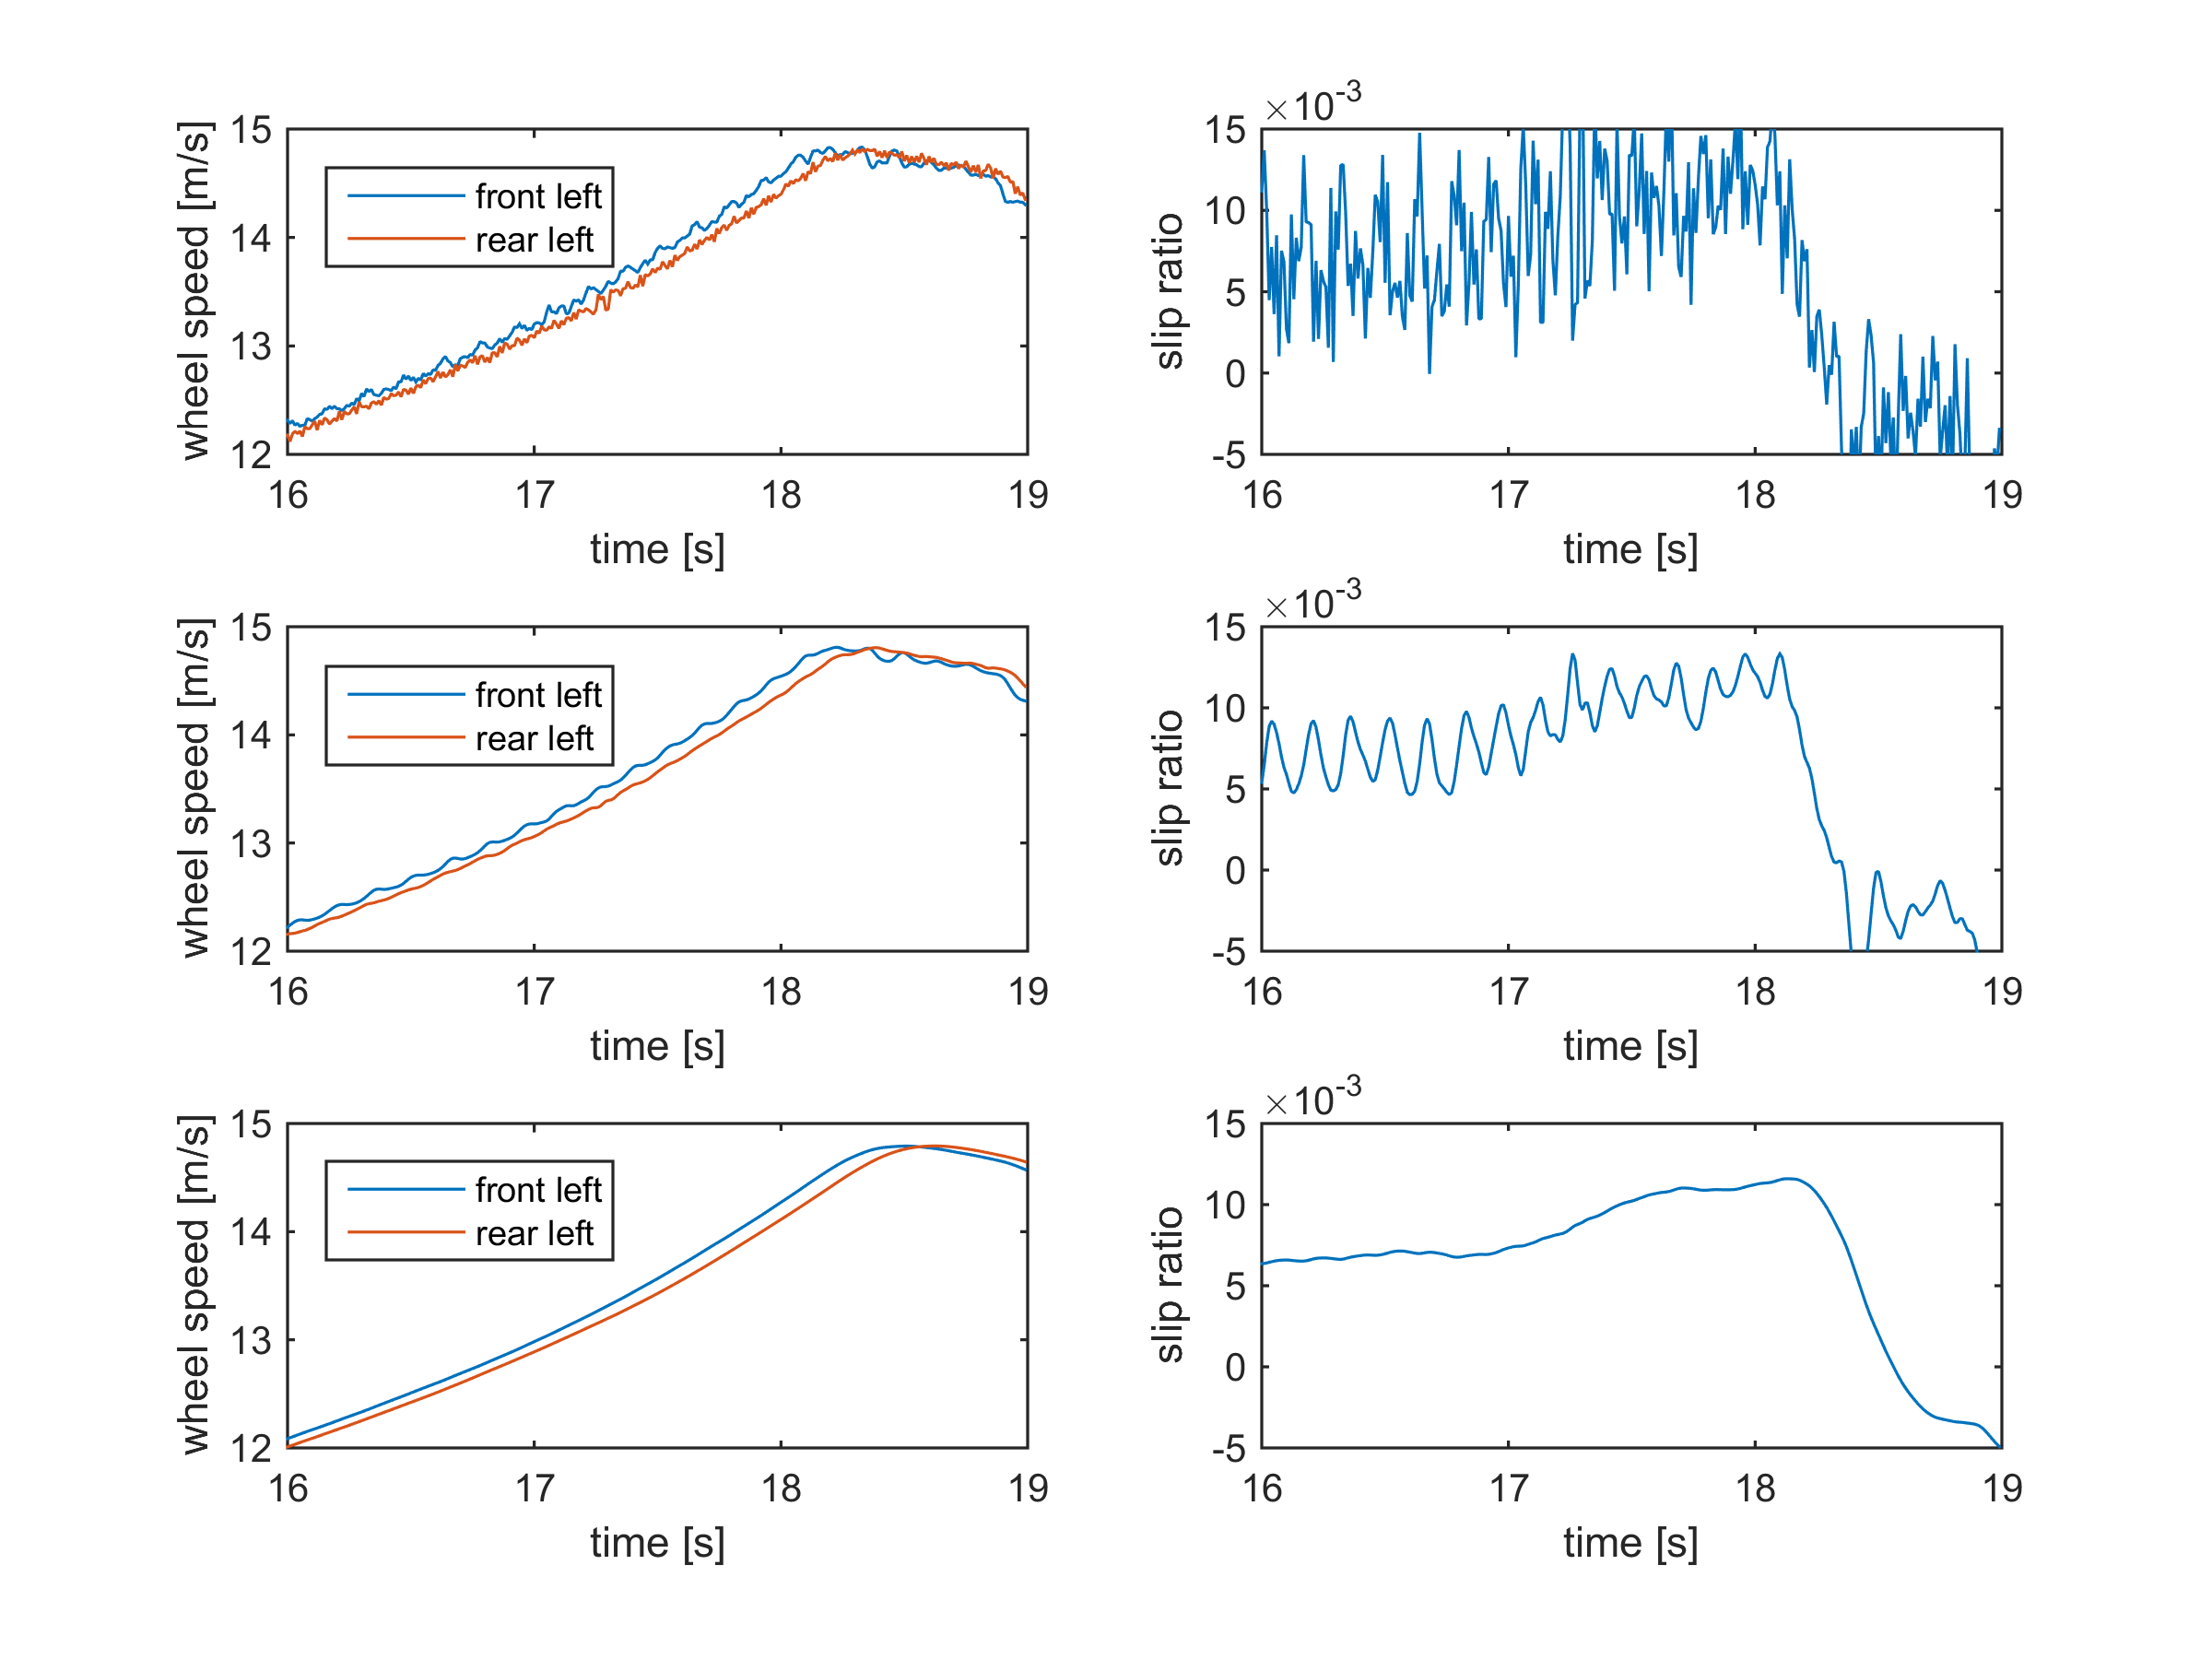
\includegraphics[width=0.8\textwidth]{Pictures/wheel_speed_and_slip}
	\caption {Wheel speeds and slips for different filters.}
	\label{wheel_speed_and_slip}
\end{figure}


Another concrete problem that arises when calculating the slip ratio, is that the radius for each wheel on a vehicle can be different, e.g. when the air pressure of a tire drops slightly over time. The wheel speed from the CAN bus will in this case be wrong, leading to a offset in the slip ratio calculations.

\todo{Skriva något fint om kraften med slip angle} The force/slip should be smaller when the slip angle is larger. In other words, when we have more lateral force, the longitudinal force will be smaller.

\subsection{Normal force}

The amount of both longitudinal and lateral force generated from tire depends on the normal force acting on the tire. The force generated by a tire is linearly proportional to the normal force on the tire
\begin{equation}
	F = F_{z}\mu_{0}
\end{equation}
Where the normalized force $ \mu_{0} $, never can exceed the friction between the tire and road
\begin{equation}
	\mu_{0} \leq \mu
\end{equation}
It is therefore important to know the loaded weight on each tire in every instant. This is done by the dynamic weight distribution calculations explained in section \ref{normal_force}. These calculations are rather simplified, where the difference in chassis stiffness between front and back is not considered. These chassis stiffness's are vehicle specific and hard to estimate. 

This means that the maximum longitudinal force obtained by either the vehicle model or the tire force model, can never be larger than the normal force multiplied by the tire/road friction coefficient, which can be helpful when unreasonable values are obtained. 

\section{Estimating the friction coefficient}

\section{Other methods}

\subsection{Slip-slope friction model}

One friction model that is frequently used and referred to in research papers is the so called slip-slope friction model. The models general idea is that the maximum tire/road friction available can be decided due to its dependency on the slope from the slip-force curve in the linear region. This slip-force curve has the same characteristics as the slip-friction coefficient curve seen in Figure \ref{fric_slip}. 
\begin{equation}
\dfrac{F_{x}}{F_{z}} = k \cdot \kappa
\end{equation}
Where $ F_{x} $ and $ F_{z} $ is the estimated longitudinal and normal force acting on a tire depending on input values. The slip-slope can be estimated with for example recursive least square fitting.
